\documentclass[12pt]{report}
%\documentclass[12pt,twoside]{report}
\usepackage[utf8]{inputenc}
%\usepackage{amsmath}
%\usepackage{amsfonts}
%\usepackage{amssymb}
\usepackage{caption}
\usepackage{subcaption}
\usepackage{graphicx}
\graphicspath{ {Images/} }

\makeatletter
\def\@@acrodef{\@ifstar\@acrodefs\@acrodef}
\newtoks\acro@list
\newcommand{\@acrodef}[2]{%
	\global\acro@list=\expandafter{\the\acro@list\@elt{#1}{#2}}%
	\global\@namedef{acro@#1}{n{#1}{#2}}}
\newtoks\acro@resetlist
\newcommand{\@acrodefs}[2]{%
	\global\acro@resetlist=\expandafter{\the\acro@resetlist\@elt{#1}}%
	\@acrodef{#1}{#2}}
\def\acro@doresetlist{\begingroup
	\def\@elt##1{\expandafter\expandafter\expandafter
		\acro@reset\csname acro@##1\endcsname}\the\acro@resetlist\endgroup}
\def\acro@reset#1#2#3{\global\@namedef{acro@#2}{n{#2}{#3}}}
\newcommand{\acro}[1]{\expandafter\expandafter\expandafter
	\use@acro\csname acro@#1\endcsname}
\def\use@acro#1#2#3{\ifx n#1
	#3 (#2)\global\@namedef{acro@#2}{o{#2}{#3}}%
	\else
	#2%
	\fi}
\newcommand{\listofacronyms}[1][tabular]{%
	\begingroup\def\@elt##1##2{##1&##2\\}%
	\@ifundefined{chapter}{\section*}{\chapter*}{\listacronymname}
	\noindent\begin{#1}{@{}p{6em}p{\dimexpr\columnwidth-2\tabcolsep-6em\relax}@{}}
		\the\acro@list
	\end{#1}\endgroup}
\providecommand\listacronymname{List of acronyms}
\newenvironment{acronyms}{\let\acrodef\@@acrodef}{}
\newenvironment{acronyms*}{\let\acrodef\@@acrodef}{\listofacronyms}
\def\g@preto@macro#1#2{\toks0=\expandafter{#1}%
	\toks2={#2}\xdef#1{\the\toks2 \the\toks0 }}
\@ifundefined{chapter}
{\g@preto@macro\section\acro@doresetlist}
{\g@preto@macro\chapter\acro@doresetlist}
\makeatother

%\usepackage[a4paper,width=150mm,top=25mm,bottom=25mm]{geometry}

\usepackage{fancyhdr}
\pagestyle{fancy}

\fancyhead{}
\fancyhead[RO,LE]{Thesis Title}
\fancyfoot{}
\fancyfoot[LE,RO]{\thepage}
%\fancyfoot[LO,CE]{Chapter \thechapter}
%\fancyfoot[CO,RE]{Author Name}

%\usepackage{biblatex}
%\addbibresource{references.bib}




%TEXT\parencite[see][p10]{latexcompanion}
%TEXT\parencite[compare][]{knuthwebsite}
%TEXT\parencite[e.g.][page 300]{einstein}

\title{
	{MeerKat Operator Manual}\\
	{\large SARAO}\\
	\vspace{1.5cm}
	{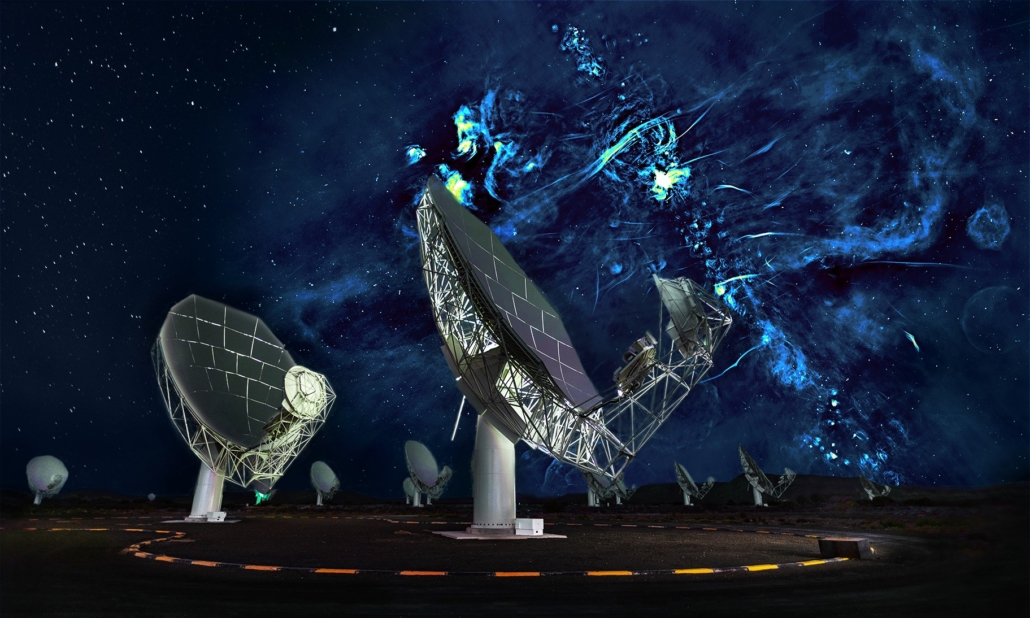
\includegraphics[width=16cm]{cover.jpg}}
}
\vspace{1.5cm}
\vspace{1.5cm}
\vspace{1.5cm}
\vspace{1.5cm}
\vfill
\author{Telescope Operators}
\date{}

\begin{document}
\maketitle
 
 
 \chapter*{Preface}

This manual is designed to help new users (i.e Students,Visitors, ) of the MeerKat Radio Telescope\cite{} to link and to undestand basic operational procedures\cite{}, and scientific procedures\cite{} that are being used to carry out scientific observations.  The complexity of the instrument requires many software interfaces for instrument setup, scheduling, monitorig and maintenace management. \\
\\
 Most of the operational terminologies and commands can only be understood by people in the operations and commissioning divisions of SARAO, thus the document bridges that gap.  The sientific community is more interested in underlying scientific methods, validation and qualification procedures that are the ultimate goal of all the operational activities.  
 
 \chapter*{Naming Convenctions }
 The following typographical rules and standards \cite{standard1} \cite{standard2} have been adopted for this manual:
 \begin{itemize}
 	\item {} Units
 	\item {} Names of servers and computers
 	\item {} Names of software packages
 	\item {} Names of software programs
 	\item {} Command line/terminal command e.g
 	\item {} Windows command
 	\item {} Filename, e.g
 	\item {} Program option
 	\item {} Acchronyms
 	\item {} Placeholder for changeable parameters
 	\item {} Optional parameter,
 	\item{ } List of possible commands or parameters
 	
 \end{itemize}
 \begin{acronyms*}
 	\acrodef{	ABL	}{	Allocated Baseline	}
 	\acrodef{	Ac	}{	Critical Availability	}
 	\acrodef{	ADR	}{	Architecture Design Review	}
 	\acrodef{	AGN	}{	Active Galactic Nuclei	}
 	\acrodef{	Ai	}{	Inherent Availability	}
 	\acrodef{	AOR	}{	Annual Operating Requirement	}
 	\acrodef{	AR	}{	Acceptance Review	}
 	\acrodef{	BOM	}{	Bill Of Material	}
 	\acrodef{	CA	}{	Criticality Analysis	}
 	\acrodef{	CDR	}{	Critical Design Review	}
 	\acrodef{	DDR	}{	Detail Design Review	}
 	\acrodef{	D-Level	}{	Deport Level	}
 	\acrodef{	DLM	}{	Depot Level Maintenance	}
 	\acrodef{	FAT	}{	Factory Acceptance Tests	}
 	\acrodef{	FMEA	}{	Failure Modes and Effects Analysis	}
 	\acrodef{	FMECA	}{	Failure Modes, Effects and Criticality Analysis	}
 	\acrodef{	FPGA	}{	Field Programmable Gate Array	}
 	\acrodef{	FRACAS	}{	Failure Reporting and Corrective Action System	}
 	\acrodef{	GHz	}{	Giga Hertz	}
 	\acrodef{	GUI	}{	Graphical User Interface	}
 	\acrodef{	HartRAO	}{	Hartbeeshoek Radio Astronomy Observatory	}
 	\acrodef{	Hrs	}{	Hours	}
 	\acrodef{	I-Level	}{	Intermediate Level	}
 	\acrodef{	ILM	}{	Intermediate Level Maintenance	}
 	\acrodef{	ILOR	}{	Intended Learning Outcomes Report	}
 	\acrodef{	ILS	}{	Integrated Logistic Support	}
 	\acrodef{	ISO	}{	International Standards Organisation	}
 	\acrodef{	KAT-7	}{	Karoo Array Telescope, 7 array	}
 	\acrodef{	Kg	}{	Kilogram	}
 	\acrodef{	Km	}{	Kilometer	}
 	\acrodef{	L3/4/5	}{	Level 3/Level 4/Level 5	}
 	\acrodef{	LEMP	}{	Logistic Engineering Management Plan	}
 	\acrodef{	LRU	}{	Line Replaceable Unit	}
 	\acrodef{	LSA	}{	Logistic Support Analysis	}
 	\acrodef{	MBL	}{	Manufacturing Baseline	}
 	\acrodef{	MSCDR	}{	Media Selection \& Curriculum Development Report	}
 	\acrodef{	MSP	}{	Maintenance \& Support Plan	}
 	\acrodef{	MTBCF	}{	Mean Time Between Critical Failures	}
 	\acrodef{	MTBF	}{	Mean Time Between Failures	}
 	\acrodef{	MTTRc	}{	Mean Time To Repair Critical	}
 	\acrodef{	MTTRi	}{	Mean Time To Repair Inherent	}
 	\acrodef{	NQF	}{	National Qualification Framework	}
 	\acrodef{	OEM	}{	Original Equipment Manufacturer	}
 	\acrodef{	O-Level	}{	Organisational Level	}
 	\acrodef{	OLM	}{	Organisational Level Maintenance	}
 	\acrodef{	OTLR	}{	Operator Task List Report	}
 	\acrodef{	PBL	}{	Product Baseline	}
 	\acrodef{	PBS	}{	Physical Breakdown Structure	}
 	\acrodef{	PC	}{	Printed Circuit	}
 	\acrodef{	PDR	}{	Preliminary Design Review	}
    	\acrodef{PHS and T}{Packaging, Handling, Storage and Transportation	}
    \acrodef{	PPPM	}{	Preparation, Preservation, Packaging \& Marking	}
    \acrodef{	PPPR	}{	Personnel Performance Profile Report	}
    \acrodef{	PRR	}{	Production Readiness Review	}
    \acrodef{	PSS	}{	Product Supplier Support	}
    \acrodef{	QBL	}{	Qualification Baseline	}
    \acrodef{	RAM	}{	Reliability, Availability, Maintainability	}
    \acrodef{	RBL	}{	Requirements Baseline	}
    \acrodef{	Relc	}{	Reliability Critical	}
    \acrodef{	Reli	}{	Reliability Inherent	}
    \acrodef{	RF	}{	Radio Frequency	}
    \acrodef{	RFI	}{	Radio Frequency Interference	}
    \acrodef{	RM	}{	Rotation Measures	}
    \acrodef{	RR	}{	Requirements Review	}
    \acrodef{	RTS	}{	Receptor Test System	}
    \acrodef{	S and TE	}{	Support and Test Equipment	}
    \acrodef{	SAQA	}{	South African Qualifications Authority	}
    \acrodef{	SEMP	}{	System Engineering Management Plan	}
    \acrodef{	SKA	}{	Square Kilometer Array	}
    \acrodef{	S-Level	}{	Supplier Level	}
    \acrodef{	SLM	}{	Supplier Level Maintenance	}
    \acrodef{	SNR	}{	Supernova Remnants	}
    \acrodef{	SRU	}{	Shop Replaceable Unit	}
    \acrodef{	TBD	}{	To Be Determined	}
    \acrodef{	TRR	}{	Test Readiness Review	}
    \acrodef{	TSR	}{	Training Survey Report	}
    \acrodef{	TTLR	}{	Technical Task List Report	}
    \acrodef{	vs	}{	Versus	}
\end{acronyms*}
 
% \section{A}
% 
% \acro{GEOAA}
% 
% \acro{IMO}
% 
% \acro{IMO}
% 
% \acro{GEOAA}
% 
% \acro{OP}
% 
% \section{B}
% 
% \acro{OP}
 
% \listofacronyms
 
 %\chapter*{Dedication}

% \renewcommand{\headrulewidth}{0.4pt}
% \renewcommand{\footrulewidth}{0.4pt}
% \chapter*{Declaration}
 
% \chapter*{Acknowledgements}
 
  \listoffigures
  
 \tableofcontents
 \chapter{Introduction}

  \chapter{User Requirements}
 
 
  \chapter{Functional Requirements}
 
 
 \chapter{System Settings Procedures}
 
 \chapter{Chapter Three Title}

 
 \chapter{Conclusion}
 
 \appendix
 \chapter{Appendix Title}
 \begin{itemize}


\item[] \textbf{Starting your shift:}

\begin{table}[H]
	
	\label{tab:checklist}
	\begin{tabular}[b]{|p{16 cm}|} 
		\hline
 Did you read the handover on OPS-CATALYST?\\
\hline
Did you read the Notice board?\\
\hline
Have you reserved antennas for site maintenance?\\
\hline
Will the sync epoch time suffice for the current schedule block?\\
\hline
Have you opened mattermost communications tool.\\
\hline
Did you run AP Meerkat status script to check availability of AP?\\
\hline
	
	\end{tabular}
\end{table}

 


\item[] \textbf{Subarray Configurations:
}
\begin{table}[H]
	
	\label{tab:checklist}
	\begin{tabular}[b]{|p{16 cm}|} 
		\hline
	Is the band, data product,dump rate,cbf,sdp and USE as per calendar request?\\
	\hline
	Have you run reset attenuation after adding antennas from maintenance?\\
	\hline
	Have all antennas calibrated for delays? if not, repeat and/or mark faulty ones?\\
	\hline
	Have you verified if phase-up must be run from calendar request?\\
	\hline
	
		
	\end{tabular}
\end{table}


 
 

\item[] \textbf{Observation:
}
\begin{table}[H]
	
	\label{tab:checklist}
	\begin{tabular}[b]{|p{16 cm}|} 
		\hline
 Is the dryrun valid, if not consult AOD\\
	\hline
	Are signal displays plotting?\\
	\hline
	
	Do you follow the progress report of the observation\\
	\hline
	Are observation files closed without errors\\
	\hline
	Is the observation file in the archive?\\
	\hline
	Have you checked the cal report and conducted the QA?\\
	\hline
	Have you opened JIRAs for encountered system problems?\\
	\hline
	Have you created/closed any timeloss logs on the telescope?\\
	\hline
	Have you updated the observation document and Operations Minutes?\\
	\hline
	
	
	Have you updated the Ops catalyst with the number of antennas available?\\
	\hline
		
	\end{tabular}
\end{table}
\end{itemize}

 \begin{itemize}


\item[] \textbf{Starting your shift:}

\begin{table}[H]
	
	\label{tab:checklist}
	\begin{tabular}[b]{|p{16 cm}|} 
		\hline
 Did you read the handover on OPS-CATALYST?\\
\hline
Did you read the Notice board?\\
\hline
Have you reserved antennas for site maintenance?\\
\hline
Will the sync epoch time suffice for the current schedule block?\\
\hline
Have you opened mattermost communications tool.\\
\hline
Did you run AP Meerkat status script to check availability of AP?\\
\hline
	
	\end{tabular}
\end{table}

 


\item[] \textbf{Subarray Configurations:
}
\begin{table}[H]
	
	\label{tab:checklist}
	\begin{tabular}[b]{|p{16 cm}|} 
		\hline
	Is the band, data product,dump rate,cbf,sdp and USE as per calendar request?\\
	\hline
	Have you run reset attenuation after adding antennas from maintenance?\\
	\hline
	Have all antennas calibrated for delays? if not, repeat and/or mark faulty ones?\\
	\hline
	Have you verified if phase-up must be run from calendar request?\\
	\hline
	
		
	\end{tabular}
\end{table}


 
 

\item[] \textbf{Observation:
}
\begin{table}[H]
	
	\label{tab:checklist}
	\begin{tabular}[b]{|p{16 cm}|} 
		\hline
 Is the dryrun valid, if not consult AOD\\
	\hline
	Are signal displays plotting?\\
	\hline
	
	Do you follow the progress report of the observation\\
	\hline
	Are observation files closed without errors\\
	\hline
	Is the observation file in the archive?\\
	\hline
	Have you checked the cal report and conducted the QA?\\
	\hline
	Have you opened JIRAs for encountered system problems?\\
	\hline
	Have you created/closed any timeloss logs on the telescope?\\
	\hline
	Have you updated the observation document and Operations Minutes?\\
	\hline
	
	
	Have you updated the Ops catalyst with the number of antennas available?\\
	\hline
		
	\end{tabular}
\end{table}
\end{itemize}

 
\bibliographystyle{plain}
\bibliography{references} 
\end{document}